\documentclass[11pt]{article}

\usepackage[utf8]{inputenc}
\usepackage[T1]{fontenc}
\usepackage{lmodern}
\usepackage[margin=1in]{geometry}
\usepackage{amsmath,amssymb}
\usepackage{booktabs}
\usepackage{tabularx}
\usepackage{array}
\usepackage{float}
\usepackage{tikz}
\usetikzlibrary{arrows.meta,positioning,calc}
\usepackage[numbers,sort&compress]{natbib}
\usepackage[hidelinks]{hyperref}

\newcommand{\lean}[1]{\texttt{#1}}
\newcommand{\code}[1]{\texttt{#1}}

\title{TWEAK Revisited: Chapman's Famous Proof Rendered in Lean}
\author{Jeff Shrager}
\date{Draft, November 2026}

\begin{document}
\sloppy
\maketitle

\begin{center}
\fbox{\parbox{0.9\linewidth}{\centering\large\textbf{Draft for Comment}\footnotemark}}
\end{center}
\footnotetext{This is a working draft. I welcome corrections,
  constructive challenges, and especially proposals for
  collaboration. Email me: \texttt{jshrager@gmail.com}.}
\medskip

\begin{abstract}
In 1985 David Chapman took the tangle of nonlinear planners that had grown
up around Sacerdoti's NOAH and distilled it into TWEAK, a planner simple
enough to prove things about. At its heart was the modal truth criterion,
a polynomial test for whether a proposition holds in every way of finishing
an incomplete plan, and a proof that the test is exactly right. The
criterion became one of the best-known results in AI planning. Here I
render Chapman's report in the Lean proof assistant, for plans without
variables. The criterion survives intact: it is necessary and sufficient
for necessary truth, and Chapman's proof strategy, building completions
that falsify the proposition, goes through almost word for word. So does
the correctness half of his correctness/completeness theorem, and the
reduction behind his intractability theorem, though what it proves is
coNP-hardness. But several of the report's smaller claims do not survive.
The criterion for \emph{possible} truth, said to be ``exactly analogous,
with all the modalities switched,'' is necessary but not sufficient. The
``white knight'' clause, which Chapman justified by an odd case involving
variables, is needed even when there are none. And the example offered of
TWEAK running forever does not run forever: TWEAK fails on it after
examining nine plans. A one-line change to the example produces the
behavior Chapman described.
\end{abstract}

\section{Introduction}
\label{sec:intro}

By the early 1980s, domain-independent planning had a celebrated success
and a reputation problem. The success was nonlinear planning: Sacerdoti's
insight that a plan under construction need not commit to the order of its
steps \citep{sacerdoti1977}, which let NOAH and its descendants solve
problems, like Sussman's ``anomaly'' \citep{sussman1975}, that defeated
planners working on one goal at a time. The reputation problem was that
nobody could say exactly why these planners worked or when they would
fail. Chapman put it plainly. He set out to copy NOAH because he needed a
planner as a subroutine, and ``four readings of [Sacerdoti] and three
misconceived implementations later, I had a planner that worked, but no
idea why'' \citep[p.~1]{chapman1985}.

His response was TWEAK \citep{chapman1985,chapman1987}: a planner stripped
to a simple representation and a short nondeterministic procedure, with
proofs. The central proof concerns a question every nonlinear planner must
answer. An incomplete plan stands for all of the complete plans that
finish it (all its \emph{completions}), and there are exponentially many
of them. Is a given proposition true at a given point in \emph{all} of
them? Chapman's modal truth criterion answers in polynomial time, by
looking for an \emph{establisher} that asserts the proposition beforehand
and checking that every step that might undo it is followed by a
\emph{white knight} that restores it. He proved that the criterion is
exactly right: sufficient and necessary. The goal-achievement procedure is
then the criterion read as a recipe, each way of making the criterion true
a way of modifying the plan, and correctness and completeness of the
planner follow from the exactness of the criterion.

Chapman described his report as the ``neat'' half of a cycle in which
scruffy, working programs are followed by rigorous reconstruction
\citep[p.~1]{chapman1985}. A proof assistant is the natural next turn of
that cycle. This paper reports what happens when Chapman's definitions and
theorems are written in Lean \citep{demoura2021}, in the style of CogLean%
\footnote{CogLean is a library of cognitive theory in the Lean proof
assistant, in which mechanisms and phenomena are stated once and theorems
relating them are machine-checked: \url{https://coglean.org}. This paper
is a self-contained application of its approach to one theory, as is
\citep{shh88revisited}.}
\citep{coglean,cogleanintro}: the paper's mechanisms are stated as
postulates with page references, and each of its claims is given a status,
proved, sharpened, reinterpreted or refuted (Table~\ref{tab:claims}). The
work is in a public repository \citep{chapman85revisited}; every result
below names the theorem that establishes it.

The formalization covers \emph{ground} plans, whose propositions contain no
variables. That is a real restriction: Chapman's criterion is stated for
plans with variables and codesignation constraints, and some of its
subtlety lives there. But as we will see, most of what is interesting about
the criterion is already present without variables, and some of the
report's claims are already wrong there.

\section{TWEAK in brief}
\label{sec:tweak}

A proposition is an atom, negated or not. A \emph{step} has preconditions
and postconditions; it \emph{asserts} its postconditions and \emph{denies}
their negations. Executing a step removes from the situation everything it
denies and adds everything it asserts \citep[p.~6]{chapman1985}. A
complete plan is a sequence of steps; an incomplete plan is a set of steps
under a partial order, and its completions are the total orders that
extend it. A proposition is \emph{necessarily} true in the input situation
of a step if it holds there in every completion, and \emph{possibly} true
if in some. A plan necessarily solves a problem when every precondition of
every step, and every goal (the preconditions of a final step), is
necessarily true where it is needed.

In the ground case the criterion reads:

\begin{quote}
\textbf{Modal truth criterion.} $p$ is necessarily true in the input
situation of step $s$ iff (i)~$p$ is in the initial situation or is
asserted by a step necessarily before $s$, and (ii)~for every step $C$
possibly before $s$ that denies $p$, there is a step $W$ necessarily
between $C$ and $s$ that asserts $p$.
\end{quote}

A step $C$ violating clause (ii) is a \emph{clobberer}; a step $W$ that
satisfies it is a \emph{white knight}. With variables, ``asserts $p$''
becomes ``asserts a proposition that codesignates with $p$ whenever $C$'s
denial does'', and ``possibly'' and ``necessarily'' range over bindings as
well as orders.

TWEAK's procedure makes an unachieved goal true by establishment (using an
existing step or the initial situation, or adding a new step, and ordering
it before $s$) and then removes each clobberer by \emph{promotion}
(ordering it after $s$), by a white knight (existing or new), or, with
variables, by \emph{separation} (forbidding a codesignation). The top
level chooses an unachieved goal, applies the procedure, and searches the
choices breadth first.

\section{The criterion, checked}
\label{sec:mtc}

The formal statement is \lean{Tweak.Ground.mtc\_iff}: for a plan whose
steps never assert and deny the same proposition, necessary truth in the
input situation of $s$ is equivalent to the criterion. The proof follows
Chapman's \citep[pp.~38--43]{chapman1985} closely enough that his lemmas
appear as named steps.

The first is the \emph{truth criterion for complete plans}: after a
sequence of steps, $p$ is true iff it was asserted somewhere, initially or
by a step, and no later step denied it (\lean{Tweak.Ground.mem\_run\_iff}).
Chapman calls this obvious and proves it by induction; so does Lean.

Sufficiency is then a short argument (\lean{Tweak.Ground.necTrue\_of\_mtc}).
In any completion, consider the steps before $s$. Every step there that
denies $p$ is followed by its white knight, which is necessarily before
$s$ and so also among them. Chapman's proof chases white knights (``there
may in turn be a step after the white knight denying $p$; but it must also
have its own white knight''); the Lean proof instead shows, by induction
from the right, that a sequence in which every denial is followed by an
assertion leaves $p$ true (\lean{Tweak.Ground.mem\_run\_of\_covered}).

Necessity is where Chapman's proof does its real work. If the criterion
fails, he \emph{constructs} a completion in which $p$ is false: if there is
no establisher, put every step that could come after $s$ after it; if
there is a clobberer $C$, put $C$ before $s$, everything that could follow
$s$ after it, and everything that could precede $C$ before $C$. His
temporal consistency lemma licenses these moves one constraint at a time.
In Lean a single lemma does all of them at once
(\lean{Tweak.Ground.exists\_completion\_rank}): give each step a rank that
never decreases along the partial order, and some completion lists the
steps in order of rank. Each of Chapman's constructions is then just a
choice of ranks. For the clobberer case, the five ranks are: steps that can
precede $C$; $C$; steps necessarily between $C$ and $s$; $s$; everything
else. In that completion the only steps between $C$ and $s$ are the ones
necessarily between them, none of which asserts $p$, so $p$ is false at
$s$ (\lean{Tweak.Ground.not\_necTrue\_of\_clobberer}). The same lemma gives
the completion lemma (\lean{Tweak.Ground.exists\_completion}) and shows
that ``necessarily before'' is just the partial order, which is what makes
the criterion polynomial (\lean{Tweak.Ground.necBefore\_iff}).

So the famous theorem is right, and the famous proof is essentially right
too: its constructions work exactly as described, and the one place it
waves its hands (the regress of white knights) is easily made precise.

With the criterion proved, correctness of TWEAK's termination test is
immediate: a plan in which every precondition and goal is necessarily true
is, in every completion, an executable sequence that achieves the goals
(\lean{Tweak.Ground.correctness}). (Completeness I have only tested: on
300 random ground domains the Python TWEAK finds a plan in the 210 that
linear search can solve, and exhausts its search space on the other 90.) And the criterion becomes a decision
procedure that Lean can run. Chapman's breakfast plan, which leaves
fetching the milk and fetching the cereal unordered, necessarily solves its
problem (\lean{Examples.breakfast\_solves}); in his Sussman-anomaly trace,
the intermediate plan has \code{(clear b)} clobbered by \code{puton a b}
exactly as he says (\lean{Examples.sussman\_clobbered}), and the final
three-step plan necessarily solves the problem
(\lean{Examples.sussman\_solves}). An executable ground TWEAK in Python
(\code{tools/tweak.py}) finds that plan after examining 390 partial plans.

\section{What the report says, and what follows}
\label{sec:claims}

Writing the theory down precisely also tests the claims made around the
main theorem. Five of them come out differently than the report says.

\subsection{White knights are needed without variables}

Chapman introduces the white-knight clause with an apology: it ``is
counter-intuitive, but it is needed, as illustrated by the previously
illustrated odd plan'' \citep[p.~9]{chapman1985}. The odd plan depends on
variables: a step denies a proposition that may or may not codesignate
with $p$, and a later step asserts that same proposition. The natural
reading is that without variables the simpler criterion suffices: an
establisher with no possibly intervening step that possibly denies $p$
\citep[p.~8]{chapman1985}.

\begin{figure}[t]
\centering
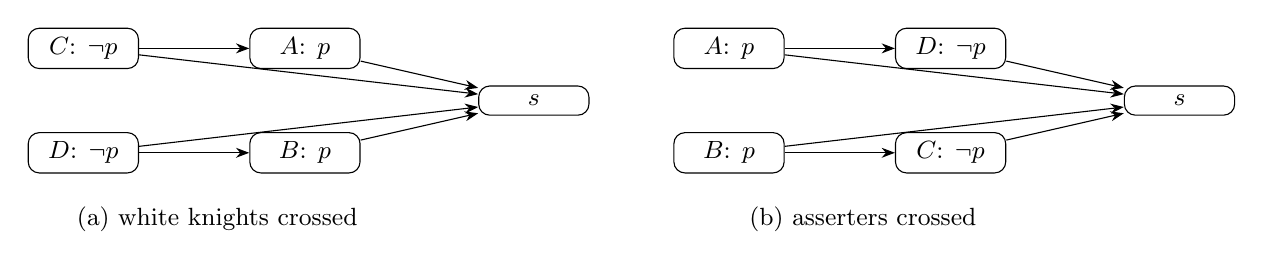
\begin{tikzpicture}[>=Stealth, node distance=8mm and 14mm,
  st/.style={draw, rounded corners, minimum width=14mm, font=\small}]
\node[st] (C) {$C$: $\neg p$};
\node[st, right=of C] (A) {$A$: $p$};
\node[st, below=of C] (D) {$D$: $\neg p$};
\node[st, right=of D] (B) {$B$: $p$};
\node[st, right=22mm of $(A)!0.5!(B)$] (S) {$s$};
\draw[->] (C) -- (A); \draw[->] (D) -- (B);
\draw[->] (A) -- (S); \draw[->] (B) -- (S);
\draw[->] (C) -- (S); \draw[->] (D) -- (S);
\node[below=3mm of D, xshift=17mm, font=\small] {(a) white knights crossed};
\begin{scope}[xshift=82mm]
\node[st] (A2) {$A$: $p$};
\node[st, right=of A2] (D2) {$D$: $\neg p$};
\node[st, below=of A2] (B2) {$B$: $p$};
\node[st, right=of B2] (C2) {$C$: $\neg p$};
\node[st, right=22mm of $(D2)!0.5!(C2)$] (S2) {$s$};
\draw[->] (A2) -- (D2); \draw[->] (B2) -- (C2);
\draw[->] (A2) -- (S2); \draw[->] (B2) -- (S2);
\draw[->] (C2) -- (S2); \draw[->] (D2) -- (S2);
\node[below=3mm of B2, xshift=17mm, font=\small] {(b) asserters crossed};
\end{scope}
\end{tikzpicture}
\caption{Two five-step ground plans. Arrows are the partial order; each
step is labeled by what it asserts. (a)~$p$ is necessarily true at $s$,
but only the white-knight clause can show it. (b)~The criterion with the
modalities switched holds, yet $p$ is false at $s$ in every completion.}
\label{fig:plans}
\end{figure}

It does not. In Figure~\ref{fig:plans}(a), two steps assert $p$ and two
deny it, with each denier ordered before one of the asserters. Whichever of
the four comes last before $s$ is an asserter, so $p$ is necessarily true.
But neither asserter can serve as the simple criterion's establisher,
because the denier not ordered before it might fall between it and $s$
(\lean{Examples.wk\_needed}). Nor does it help to read the simple criterion
generously, taking as establisher any earlier situation in which $p$ is
necessarily true, as Chapman's wording allows: for every step before $s$
there is a denier that can fall between that step and $s$
(\lean{Examples.wk\_needed\_any}). The criterion handles the plan only through
its white-knight clause, each asserter rescuing the other's denier, with a
white knight that is not the establisher. This also qualifies Chapman's
later remark that declobbering by a white knight distinct from the
establisher is ``pretty useless'' \citep[p.~32]{chapman1985}. As a way of
modifying plans it may be; as part of a test of truth it is indispensable.

\subsection{Switching the modalities does not give possible truth}

The report states the criterion for necessary truth and then adds: ``The
criterion for possible truth is exactly analogous, with all the modalities
switched (read `necessary' for `possible' and vice versa)''
\citep[p.~9]{chapman1985}. Switched, the criterion asks for an establisher
\emph{possibly} before $s$, and for every step \emph{necessarily} before
$s$ that denies $p$, a white knight \emph{possibly} between them.

Figure~\ref{fig:plans}(b) satisfies that test. Each denier has an asserter
that could come after it. But each asserter is ordered before the other
denier, so whichever of the four steps comes last is a denier, and $p$ is
false at $s$ in every completion (\lean{Examples.switched\_not\_sufficient}).
The individual white knights are each possible; what is impossible is to
have them all at once. The switched criterion is a necessary condition for
possible truth (\lean{Tweak.Ground.switched\_of\_possTrue}), but not a
criterion. The asymmetry is not an accident of the example. Necessary
truth can be checked one clobberer at a time because Chapman's completions
can falsify $p$ by attending to a single clobberer. Possible truth needs a
single completion that satisfies every white-knight requirement
simultaneously, and nothing in the switched criterion asks for that.

\subsection{The looping example fails instead}

The outcomes lemma says that TWEAK can succeed, fail, or run forever. For
the third case the report gives a problem: initially $\neg g$ and $\neg h$;
goals $g$ and $h$; one operator with precondition $\neg h$ and
postcondition $g$, another with precondition $\neg g$ and postcondition
$h$. ``TWEAK loops on this problem, building plans that are longer and
longer chains of steps that alternately assert $g$ and $h$''
\citep[p.~44]{chapman1985}.

The problem indeed has no solution (\lean{Examples.loop\_unsolvable}), as
the completeness theorem requires of any problem on which TWEAK does not
succeed. But TWEAK does not loop on it. No operator asserts $\neg g$ or
$\neg h$ (\lean{Examples.loop\_no\_reassert}), so the only establisher of
either precondition is the initial situation, and no white knight can
protect it. Once the plan has one step of each kind, each clobbers the
other's precondition, promotion in either direction makes the other
clobbering necessary, and no further modification applies. Nor does
anything add more steps: the final goals, once established, stay
established, because nothing denies $g$ or $h$. The search space is
finite. Breadth-first TWEAK exhausts it after nine plans, whatever bound is
placed on plan size (\code{tools/tweak.py}), and reports failure.

What Chapman describes happens if the operators' conditions are moved into
their postconditions: one operator asserts $g$ and $\neg h$, the other $h$
and $\neg g$. Now each new step clobbers the other goal and needs a white
knight, which clobbers the first goal and needs a white knight of its own.
That problem is also unsolvable (\lean{Examples.loop2\_unsolvable}), and
the search grows without bound: 5, 17, 93 and 813 plans with plan sizes
bounded at 2, 4, 6 and 8 steps. The outcomes lemma is true, then, but its
example of nontermination is an example of failure.

\subsection{Intractability is coNP-hardness}

Chapman's intractability theorem says that once actions can be
conditional, deciding necessary truth is NP-hard
\citep[pp.~23, 45--46]{chapman1985}. The proof, which he credits to Stan
Rosenschein, encodes a formula in disjunctive normal form as a plan: for
each atom a step that makes it true, for each clause a conditional step
that asserts \emph{satisfied} if the clause holds, and a flag,
\emph{checking}, raised before all the clause steps and lowered after,
which makes any atom step that falls between them assert \emph{satisfied}
too. The completions with no atom step inside the checking window are
exactly the truth assignments, so \emph{satisfied} is necessarily true at
the end iff every assignment satisfies some clause.

The construction is correct (\lean{Tweak.Extended.reduction\_correct});
its formal proof is the longest in the repository, mostly bookkeeping
about which steps precede which in a completion. What it reduces from is
\emph{validity} of DNF formulas, which is coNP-complete. So the reduction
shows that necessary truth with conditional actions is coNP-hard. It is
NP-hard only in the weaker sense of Turing reductions; under many-one
reductions the NP-hard problem is the complement, whether \emph{satisfied}
is possibly false. The substance of Chapman's point, that the frame problem
becomes intractable once effects depend on the situation, is untouched.

\subsection{Synergy}

The report's account of \emph{why} richer actions break the criterion is
an example credited to David McAllester \citep[pp.~21--22]{chapman1985}: a
block with room for two, and three unordered steps each of which puts a
block on it. Is there room before the first? No single step denies it,
since from the establishing situation each uses up only one unit of room.
Yet two of them together use up both. Lean confirms all three parts: no
step denies ``there is room'' from the initial situation
(\lean{Synergy.no\_single\_denier}), but each step denies it in the
situation any other step leaves (\lean{Synergy.second\_denies}), and in one
completion there is no room (\lean{Synergy.synergy}). The middle theorem
locates the failure. With situation-dependent effects, ``denies'' is no
longer a property of a step but of a step in a situation, and the
criterion's clobberer test, which inspects steps one at a time, has nothing
fixed to inspect.

\begin{table}[t]
\centering
\small
\begin{tabularx}{\linewidth}{>{\raggedright\arraybackslash}p{0.38\linewidth}X}
\toprule
Claim (page) & Status \\
\midrule
Truth criterion for complete plans (39) & proved (\lean{mem\_run\_iff}) \\
Completion and temporal consistency lemmas (40) & proved, ground (\lean{exists\_completion\_rank}) \\
Modal truth criterion (9, 41--43) & proved, ground (\lean{mtc\_iff}); with variables open \\
Possible truth by switching modalities (9) & refuted: necessary, not sufficient \\
White-knight clause needed because of variables (8--9) & sharpened: needed without them \\
Criterion is polynomial (9) & reinterpreted: decided by the criterion; bound not formalized \\
Correctness of TWEAK (13) & proved (\lean{correctness}) \\
Completeness of TWEAK (13) & checked empirically on 300 random ground domains; open in Lean \\
Nontermination example (44) & refuted as printed (TWEAK fails); corrected version loops \\
Sussman anomaly trace (14--17) & proved at the checked stages \\
Synergy breaks the criterion (21--22) & proved \\
Intractability theorem (23, 45--46) & reduction proved; the result is coNP-hardness \\
Undecidability theorems (13, 24, 44--47) & not formalized \\
\bottomrule
\end{tabularx}
\caption{The report's claims and their status in the formalization. Full
details, with theorem names, are in \code{notes/CLAIMS.md}
\citep{chapman85revisited}.}
\label{tab:claims}
\end{table}

\section{Discussion}
\label{sec:discussion}

The modal truth criterion held up. That is worth saying first, because
this kind of exercise is more often reported for what it breaks. Chapman's
theorem is right in the ground case, and his proof, written in a technical
report by a master's student, maps onto a machine-checked proof with
little more than a change of notation. The one genuinely new device in the
Lean version, the ranked completion, is a compression of his own
constructions rather than a repair.

What did not hold up is instructive in a different way. Each failure was a
claim that the report did not prove: the possible-truth criterion was
asserted by analogy; the need for white knights was motivated by an
example rather than examined; the looping example was described rather
than run; and the complexity class followed from naming the problem
reduced from rather than checking which way the reduction goes. None of
these touches the main theorem, and none would have been caught by
reading, since each is plausible on its face. They were caught because
stating them precisely enough for Lean (or for a program with the same
semantics) forced the question each one had skipped.

The report's influence makes these details matter. Later work examined
what role truth criteria actually play in planning
\citep{kambhampati1996}, gave planners whose completeness proofs do not
rest on such a criterion \citep{mcallester1991}, and analyzed the
complexity of reasoning about partially ordered plans in detail
\citep{nebel1994}. I have not tried to establish here which of the points
above were noticed in that literature; readers who know it better will be
able to say.

\paragraph{Limitations.} Everything here is for ground plans. Chapman's
criterion is stated with variables and codesignation constraints, and the
codesignation half of his proof, with its two consistency lemmas and the
codesignation implication in the white-knight clause, is the next tier of
the formalization. The completeness of TWEAK is checked only empirically,
against linear search on random small domains; a formal proof needs the
goal-achievement procedure itself in Lean. The undecidability theorems are
not formalized. The statements about TWEAK's search (the nine plans, the
unbounded growth) are about my reimplementation of the procedure in
appendix~B of the report, not about Chapman's program.

\section{Conclusion}

Chapman wanted a planner he could trust as a subroutine, and built one by
proving that its central test was exactly right. Forty years on, a proof
assistant agrees with him about that test. It disagrees about some of what
he said around it: possible truth is not the mirror image of necessary
truth, white knights earn their place even without variables, the example
of a planner running forever is an example of one giving up, and the
intractability he found is coNP-hardness. None of this needed new
mathematics. It needed the theory written down precisely enough that its
consequences could be checked, which is exactly the move Chapman made with
NOAH, carried one step further.

\section*{Availability}

All definitions and theorems are in Chapman85Revisited
\citep{chapman85revisited} (Lean 4.35.0, core library only). Every theorem
is fully proved, with no \code{sorry}, and depends only on Lean's standard
axioms. The Python programs in \code{tools/} have the same semantics as the
Lean definitions: \code{mtc\_check.py} checks the ground criterion against
brute force on 42,345 random queries and found the witnesses used above;
\code{tweak.py} is an executable ground TWEAK.

\section*{Acknowledgements}

Almost all of the Lean programming was accomplished by Claude Code with
extensive guidance from the author. Papers and presentations were
initially drafted by LLMs and then substantially rewritten by the author.
Any remaining errors, including hallucinations, are the author's alone.

\bibliographystyle{unsrtnat}
\bibliography{refs}

\end{document}
